% !TeX root = main.tex
\clearpage
\subsection{A4: Modelo C4 y diagramas de secuencia}
\label{sec:fase5-a4}

\subsubsection{Alcance, niveles y estado del diseño}

El modelo representa la solución completa de BookStack CNA y desarrolla
la evolución de la arquitectura de la Figura~\ref{fig:arquitectura_logica}.
La figura original conserva la línea base del TP I; las nuevas vistas describen
el objetivo de integración del TP II. Se contrastaron las interacciones de la
sección 3.4, los requisitos de A4 y las pruebas P30--P32 de la consigna.

En C4, el nivel 1 muestra personas y sistemas; el nivel 2 abre el sistema
en aplicaciones y almacenes. Un contenedor C4 es una unidad de ejecución o
persistencia y no necesariamente un contenedor Docker. BookStack con PHP-FPM
y MariaDB pertenecen al nivel 2 aunque continúen como servicios del sistema
operativo. Las agrupaciones por VM añaden la ubicación prevista que solicita
el trabajo sin convertir el contexto de nivel 1 en un inventario de procesos.

\textbf{Estado: arquitectura objetivo de Fase 5.} El monolito de VM-1 y SSH
por su interfaz Solo host están verificados. VM-2, Swarm, microservicios,
almacenes nuevos y observabilidad se representan como diseño pendiente de
implementación. No se atribuye funcionamiento real a los flujos por haberlos
dibujado. Al finalizar Fase 6 se cotejarán estas vistas con los servicios,
puertos, reglas de red, volúmenes y versiones efectivamente desplegados.

Las decisiones proceden de ADR-006 a ADR-010 y de los contratos de A3.
El sistema en estudio abarca tanto el monolito como su extensión CNA:
BookStack no se modela como un sistema externo de esta misma plataforma.
El nivel 2 se presenta en dos láminas complementarias para distinguir el
flujo funcional de la telemetría; no son dos arquitecturas distintas.

\subsubsection{C4 nivel 1: contexto}

La Figura~\ref{fig:a4-c4-contexto} identifica al editor o lector, al consumidor
de API y al operador. Los primeros utilizan HTTPS en el gateway; el operador
administra los nodos y consulta paneles por la red privada. La caja central
resume el propósito de la plataforma y su frontera de responsabilidad.

\begin{figure}[H]
\centering
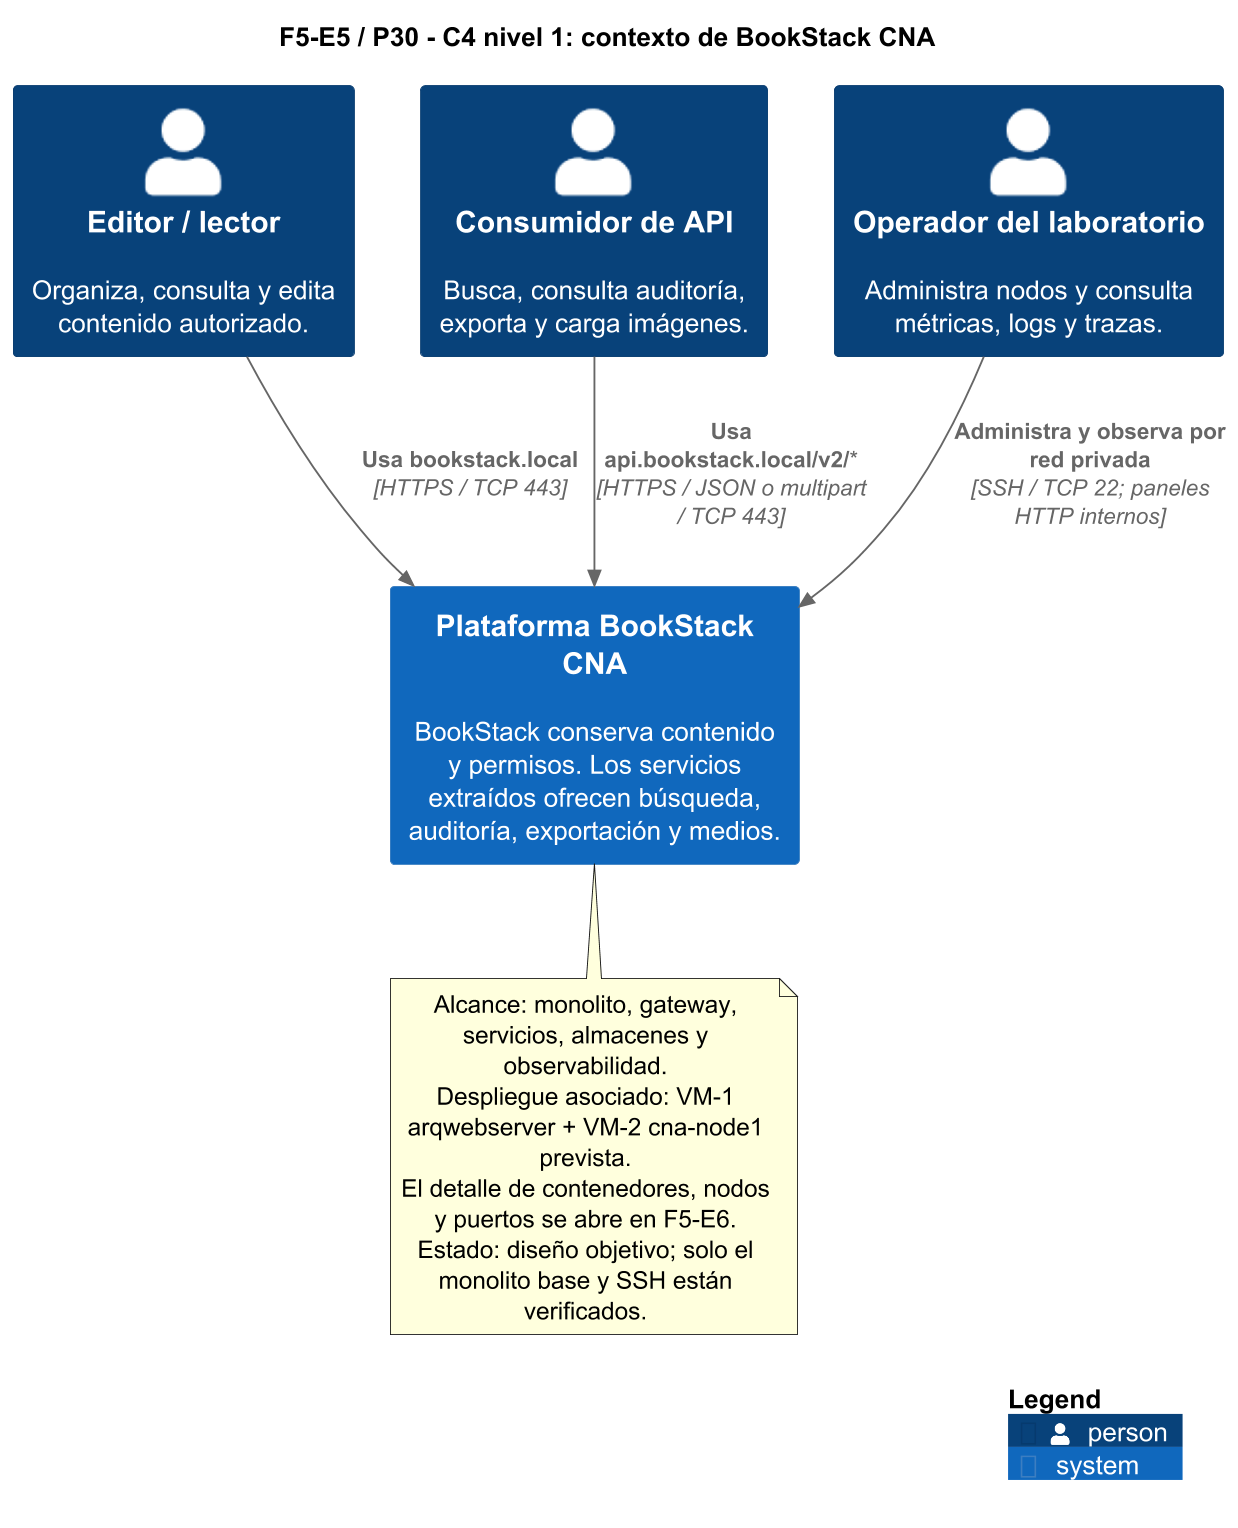
\includegraphics[width=0.71\textwidth,height=0.65\textheight,keepaspectratio]{../../../cna/docs/evidencias/fase5/a4/F5-E5-c4-contexto.png}
\caption{F5-E5 / P30. C4 nivel 1: actores y contexto de la plataforma BookStack CNA.}
\label{fig:a4-c4-contexto}
\end{figure}

\clearpage
\subsubsection{C4 nivel 2: aplicaciones, datos y operación}

Las Figuras~\ref{fig:a4-c4-contenedores} y~\ref{fig:a4-c4-operacion}
agregan nodos, protocolos y puertos. VM-1 conserva Nginx, PHP-FPM y MariaDB;
se prevé manager Swarm en \texttt{drain}. VM-2 alojará servicios, workers,
puente, broker, persistencia y observabilidad. Antes se medirá RAM y se
fijarán límites; asignar 4 GB no demuestra capacidad.

S1, S2 y el puente usan bases y roles exclusivos en PostgreSQL. S3 usa Redis
y MinIO; S4, su propio bucket. NATS distribuye eventos y no duplica la cola
ejecutable de S3. Los servicios no acceden a MariaDB.

La vista operativa incluye Prometheus, Grafana, Loki, Collector, Jaeger,
exporters y un agente de logs en VM-1. Repite referencias de la primera
lámina, sin duplicar contenedores. No supone OTLP nativo en Nginx;
la instrumentación de Webhooks se verificará sin cambiar el código del monolito.

\begin{table}[H]
\centering\small
\begin{tabularx}{\textwidth}{>{\raggedright\arraybackslash}p{3.5cm} >{\raggedright\arraybackslash}p{4.3cm} X}
\toprule
\textbf{Tramo} & \textbf{Protocolo y puerto} & \textbf{Alcance} \\
\midrule
Cliente--gateway & HTTPS/TCP 443; HTTP 80 para redirección & Entrada web; dominios del monolito y de API. \\
Operador--nodos & SSH/TCP 22 & Solo host; VM-1 verificada, VM-2 prevista. \\
Gateway--BookStack & FastCGI por socket Unix & Local en VM-1; ruta efectiva a cotejar. \\
BookStack--MariaDB & Socket local o TCP 3306 local & Transporte efectivo a verificar; sin acceso de servicios. \\
Gateway--S1/S2/S3/S4 & HTTP 8081/8082/8083/8084 hacia 8000 & Publicación privada \texttt{mode=host} propuesta. \\
BookStack--puente & HTTP 8085 hacia 8000 & Webhook y token; red privada. \\
Servicios--almacenes & SQL 5432; RESP 6379; NATS 4222; S3 HTTP 9000 & Red interna; credenciales y propiedad separadas. \\
Swarm entre nodos & TCP 2377; TCP/UDP 7946; UDP 4789 & Solo nodos privados; ESP si se cifra overlay. \\
\bottomrule
\end{tabularx}
\caption{Puertos funcionales propuestos en A4. No representan un relevamiento de sockets ni reglas de firewall ya aplicadas.}
\label{tab:a4-puertos}
\end{table}

Los puertos de telemetría y sus restricciones se detallan en la vista
operativa y en la tabla completa junto a las fuentes. VM-1 conserva
\texttt{192.168.145.129} en \texttt{ens37}; \texttt{ens33} usa DHCP.
La IP privada de VM-2 está pendiente. Un manager, un broker y volúmenes
locales no constituyen alta disponibilidad.

\clearpage
\begin{landscape}
\pdfpageattr{/Rotate 90}
\begin{figure}[p]
\centering
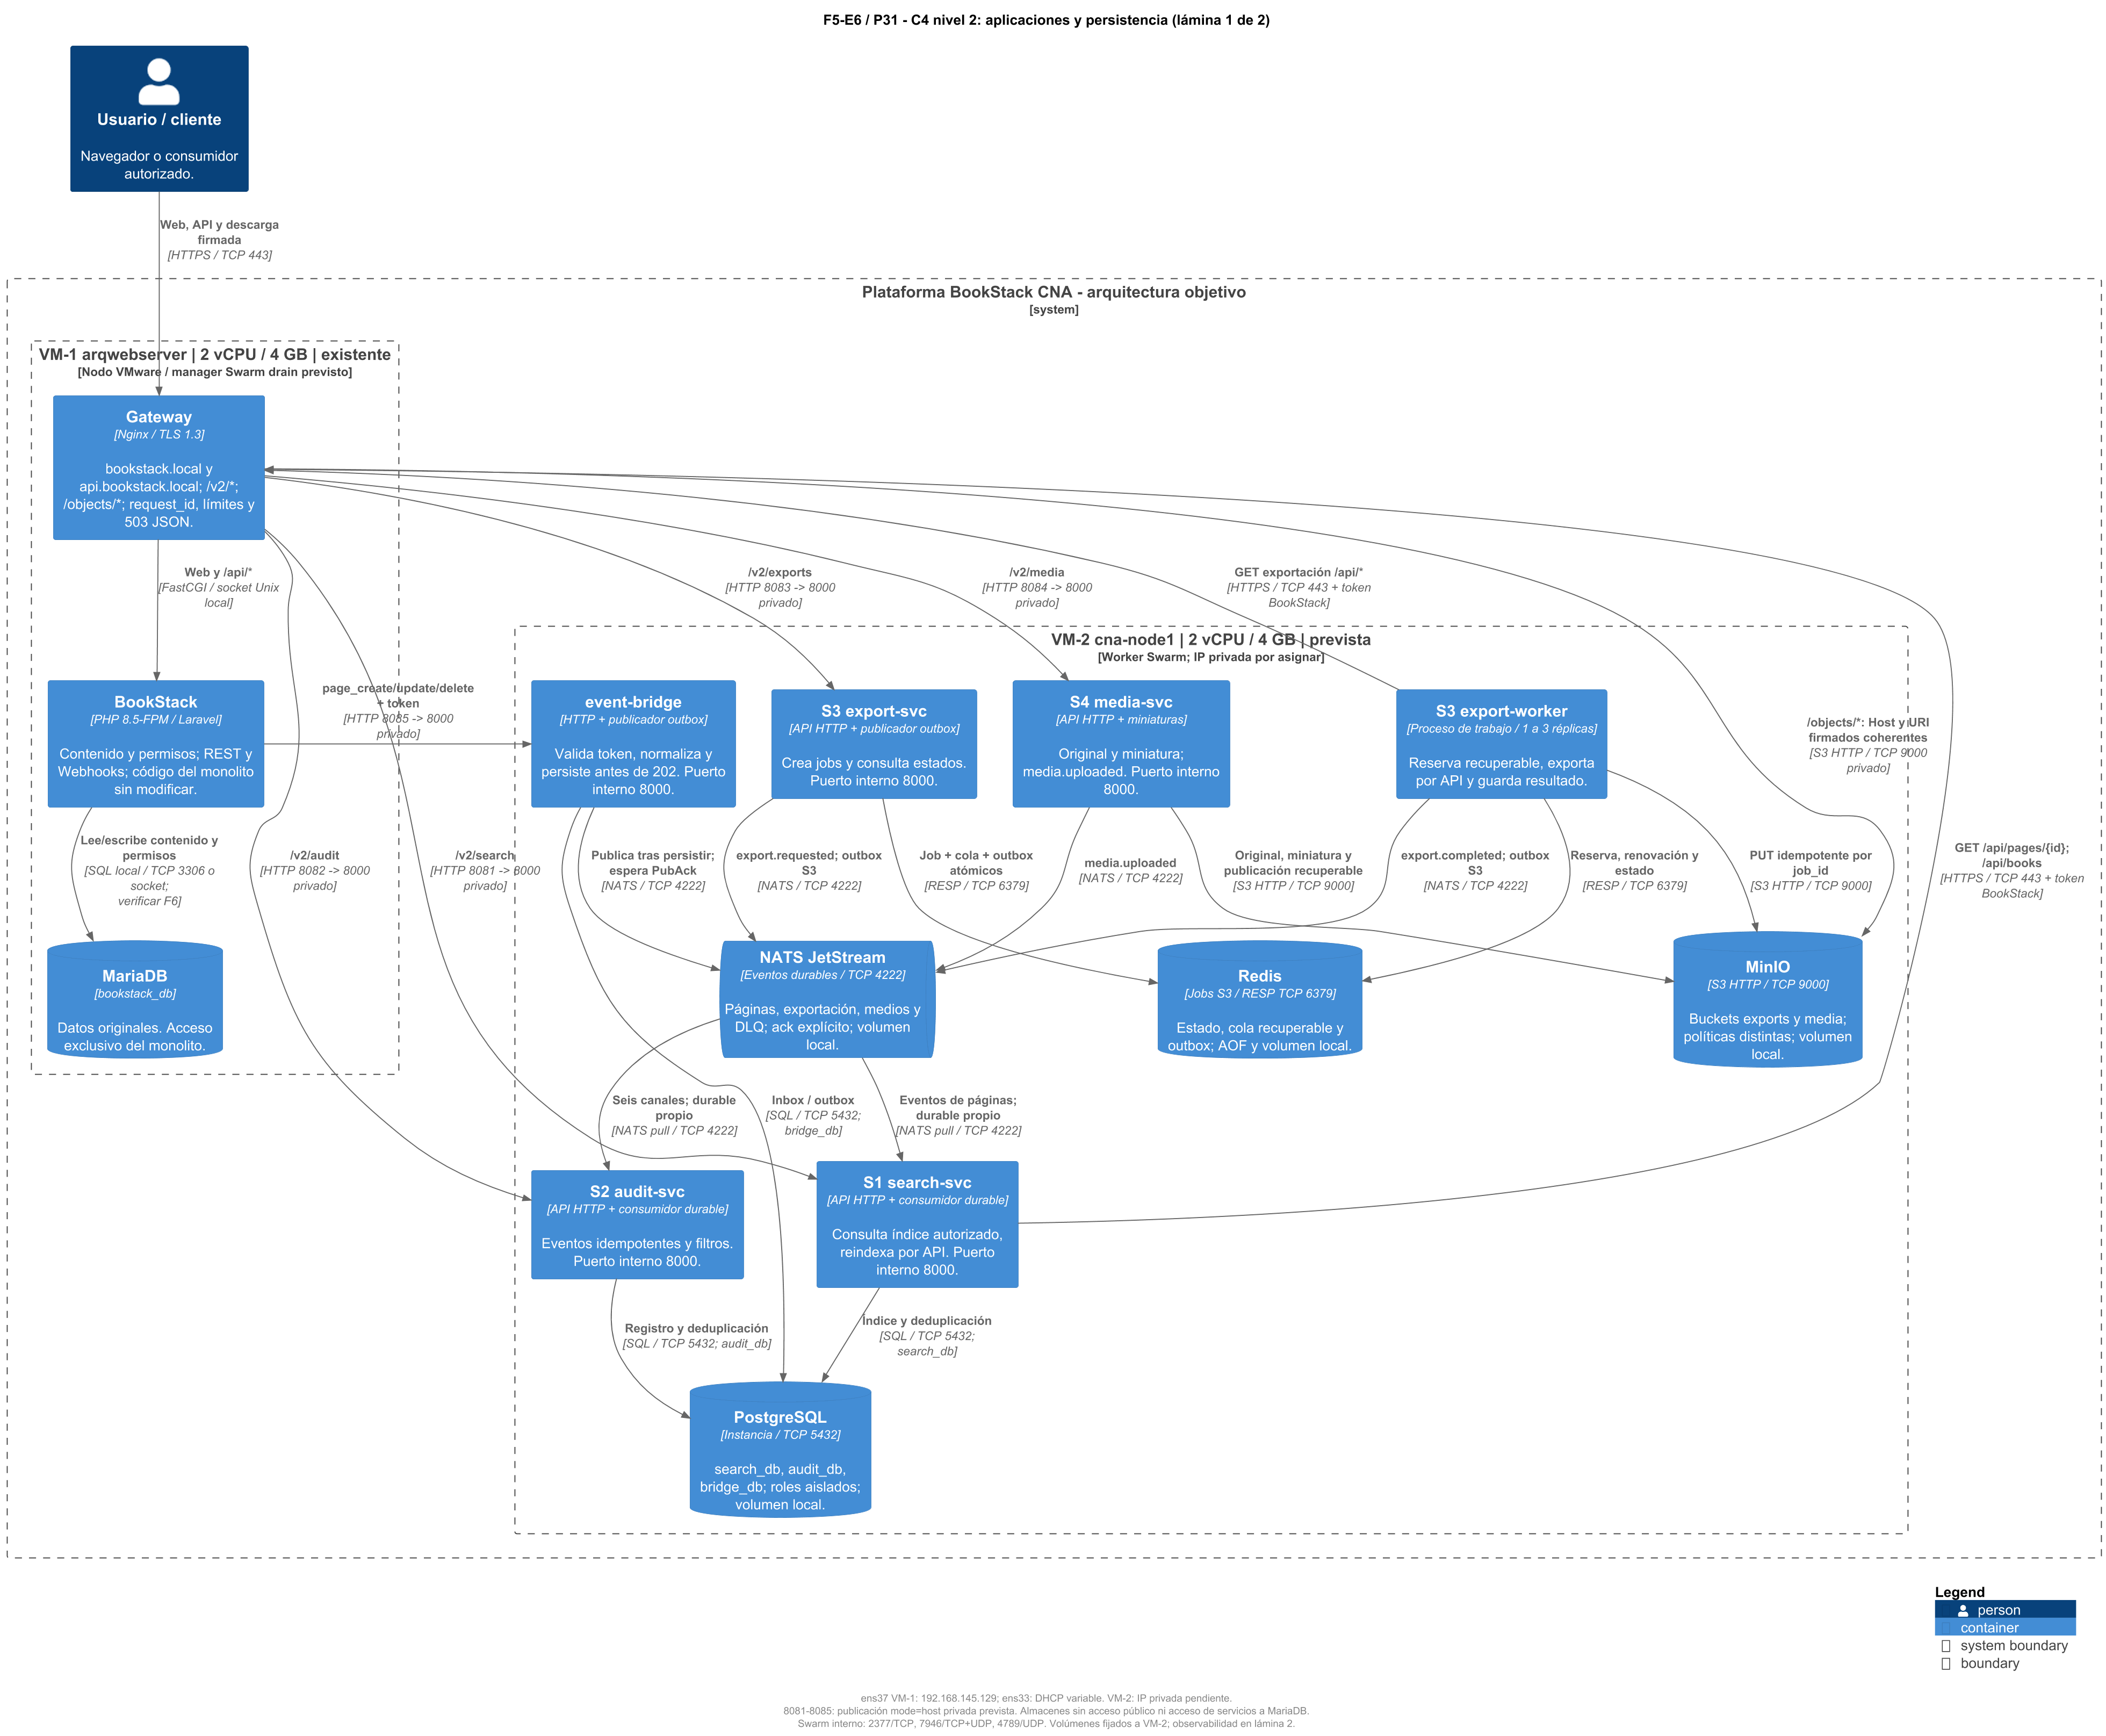
\includegraphics[width=\linewidth,height=0.86\textheight,keepaspectratio]{../../../cna/docs/evidencias/fase5/a4/F5-E6-01-c4-contenedores.png}
\caption{F5-E6 / P31. C4 nivel 2, lámina 1: aplicaciones, persistencia, nodos y comunicaciones de la arquitectura objetivo.}
\label{fig:a4-c4-contenedores}
\end{figure}
\clearpage
\begin{figure}[p]
\centering
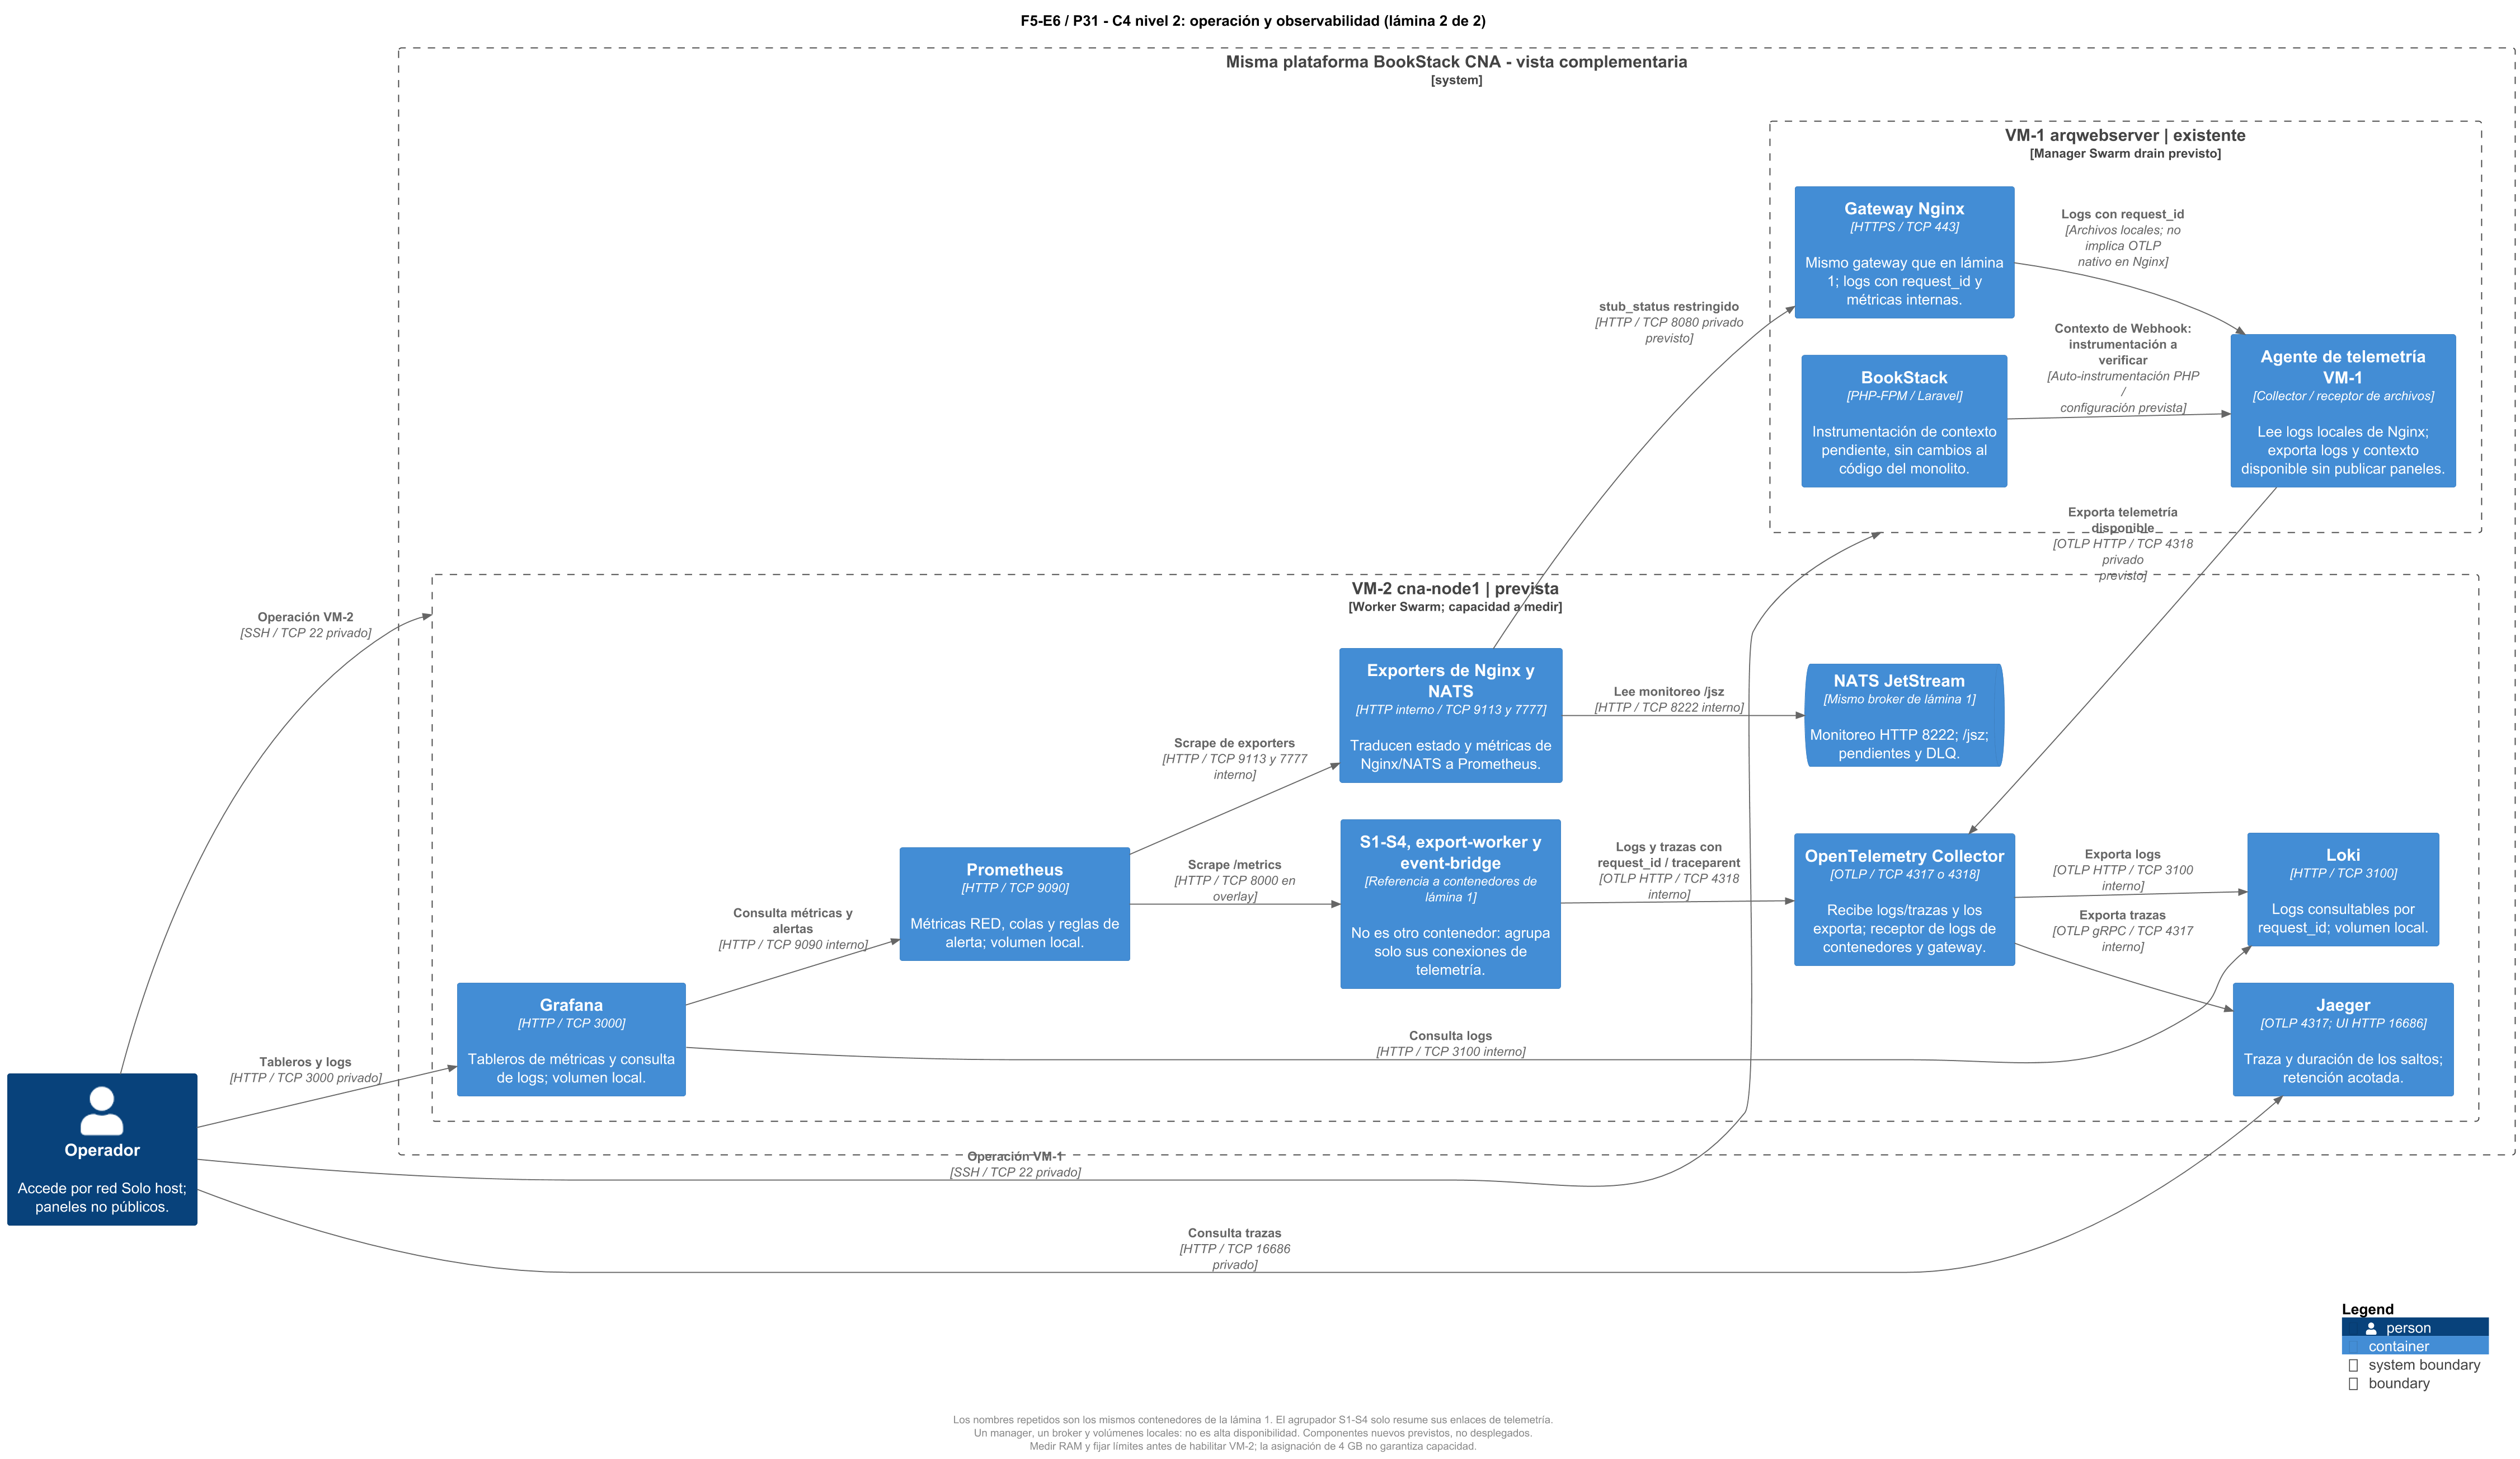
\includegraphics[width=\linewidth,height=0.86\textheight,keepaspectratio]{../../../cna/docs/evidencias/fase5/a4/F5-E6-02-c4-operacion.png}
\caption{F5-E6 / P31. C4 nivel 2, lámina 2: administración, métricas, logs y trazas previstas, complementarias a la lámina funcional.}
\label{fig:a4-c4-operacion}
\end{figure}
\clearpage
\end{landscape}
\pdfpageattr{}

\subsubsection{Tres secuencias y sus caminos de error}

Cada diagrama corresponde a una interacción obligatoria de la sección 3.4.
Se lee de arriba hacia abajo; \texttt{alt} separa alternativas y \texttt{par}
representa consumidores independientes. Edición y exportación se dividen
en dos láminas cada una para conservar legibilidad. Se mantienen tres
interacciones lógicas, no cinco casos diferentes.

\paragraph{Edición, indexación y auditoría.}
Las Figuras~\ref{fig:a4-edicion} y~\ref{fig:a4-edicion-error} siguen la edición,
el Webhook y la aceptación persistente del puente. La publicación espera
confirmación de JetStream. S1 obtiene contenido autorizado por la API y
guarda índice y deduplicación en una transacción; S2 registra el mismo evento
en su propia base. Ambos reconocen después de guardar sus efectos.
Los errores cubren entrada inválida, persistencia o broker caídos,
timeout hacia BookStack, reentrega, consumidor detenido y traslado confirmado
a DLQ. La meta de indexación menor que cinco segundos requiere medición real.

El código relevado no reprograma el Webhook si nunca llega al puente.
La recuperación del índice por API no reconstruye por sí sola la auditoría
perdida. Además, el Webhook no hereda automáticamente el identificador de la
edición: si falta, el puente inicia otra correlación. Estas limitaciones
quedan visibles y requieren tratamiento y prueba en las siguientes fases.

\paragraph{Búsqueda síncrona.}
La Figura~\ref{fig:a4-busqueda} recorre cliente, gateway, S1 e índice propio.
Incluye validación, autorización, respuesta 200 y enlaces al monolito.
Sin coincidencias devuelve una lista vacía con 200. Los caminos de error
incluyen 400, 401/403, 429 y 503 por S1 o base inaccesibles. El gateway debe
convertir los fallos del upstream al error JSON acordado y conservar
\texttt{X-Request-ID}; la consulta no accede a MariaDB.

\paragraph{Exportación por trabajos.}
Las Figuras~\ref{fig:a4-exportacion} y~\ref{fig:a4-exportacion-error}
recorren el 202 y su \texttt{job\_id}, reserva recuperable, exportación por API,
objeto en MinIO, estado \texttt{done} y descarga firmada mediante el gateway.
Los errores incluyen conflicto de clave idempotente, Redis no disponible
antes de aceptar, API o almacenamiento fallidos y caída del worker.
Un job fallido conocido se consulta con 200 y estado \texttt{failed}.
La publicación pendiente se conserva en outbox si NATS falla. Redis AOF
y volúmenes requieren validar su política real de persistencia; no se
presentan como una garantía de pérdida cero ante cualquier caída.

\clearpage
\begin{figure}[p]
\centering
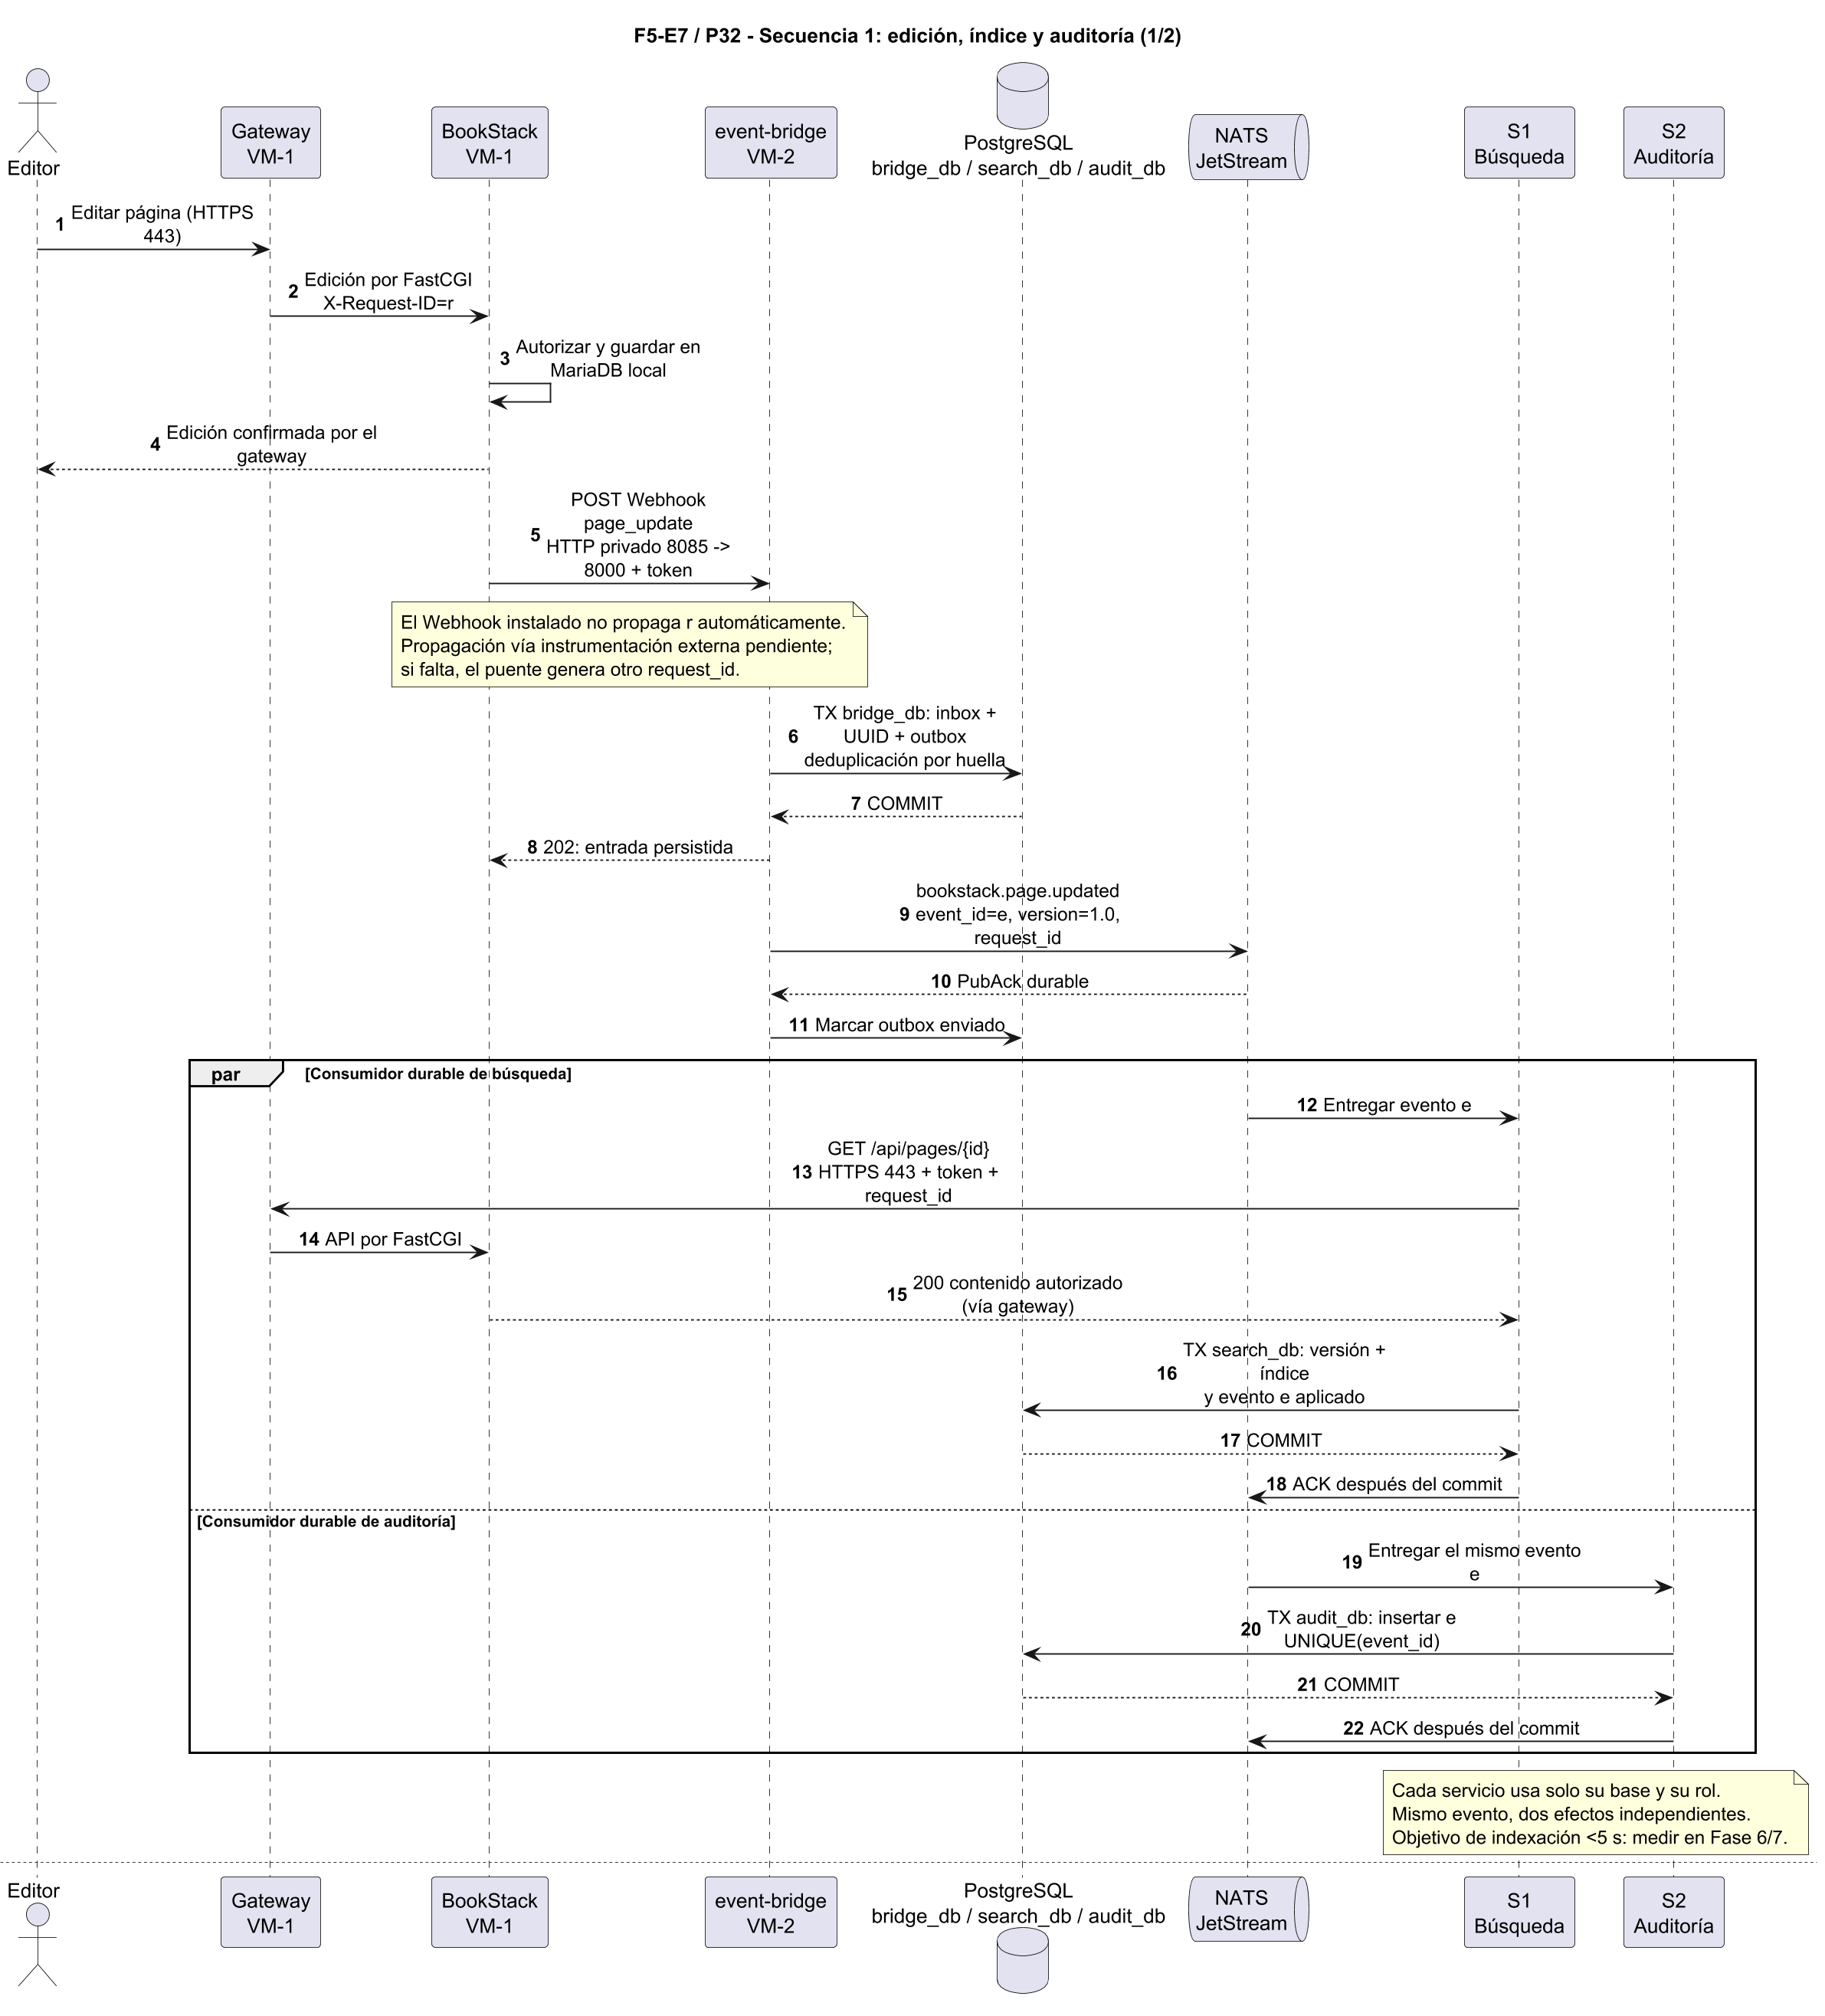
\includegraphics[width=\textwidth,height=0.88\textheight,keepaspectratio]{../../../cna/docs/evidencias/fase5/a4/F5-E7-01-edicion-indexacion.png}
\caption{F5-E7 / P32. Secuencia 1, lámina principal: edición, aceptación persistente, indexación y auditoría independientes.}
\label{fig:a4-edicion}
\end{figure}
\clearpage
\begin{figure}[p]
\centering
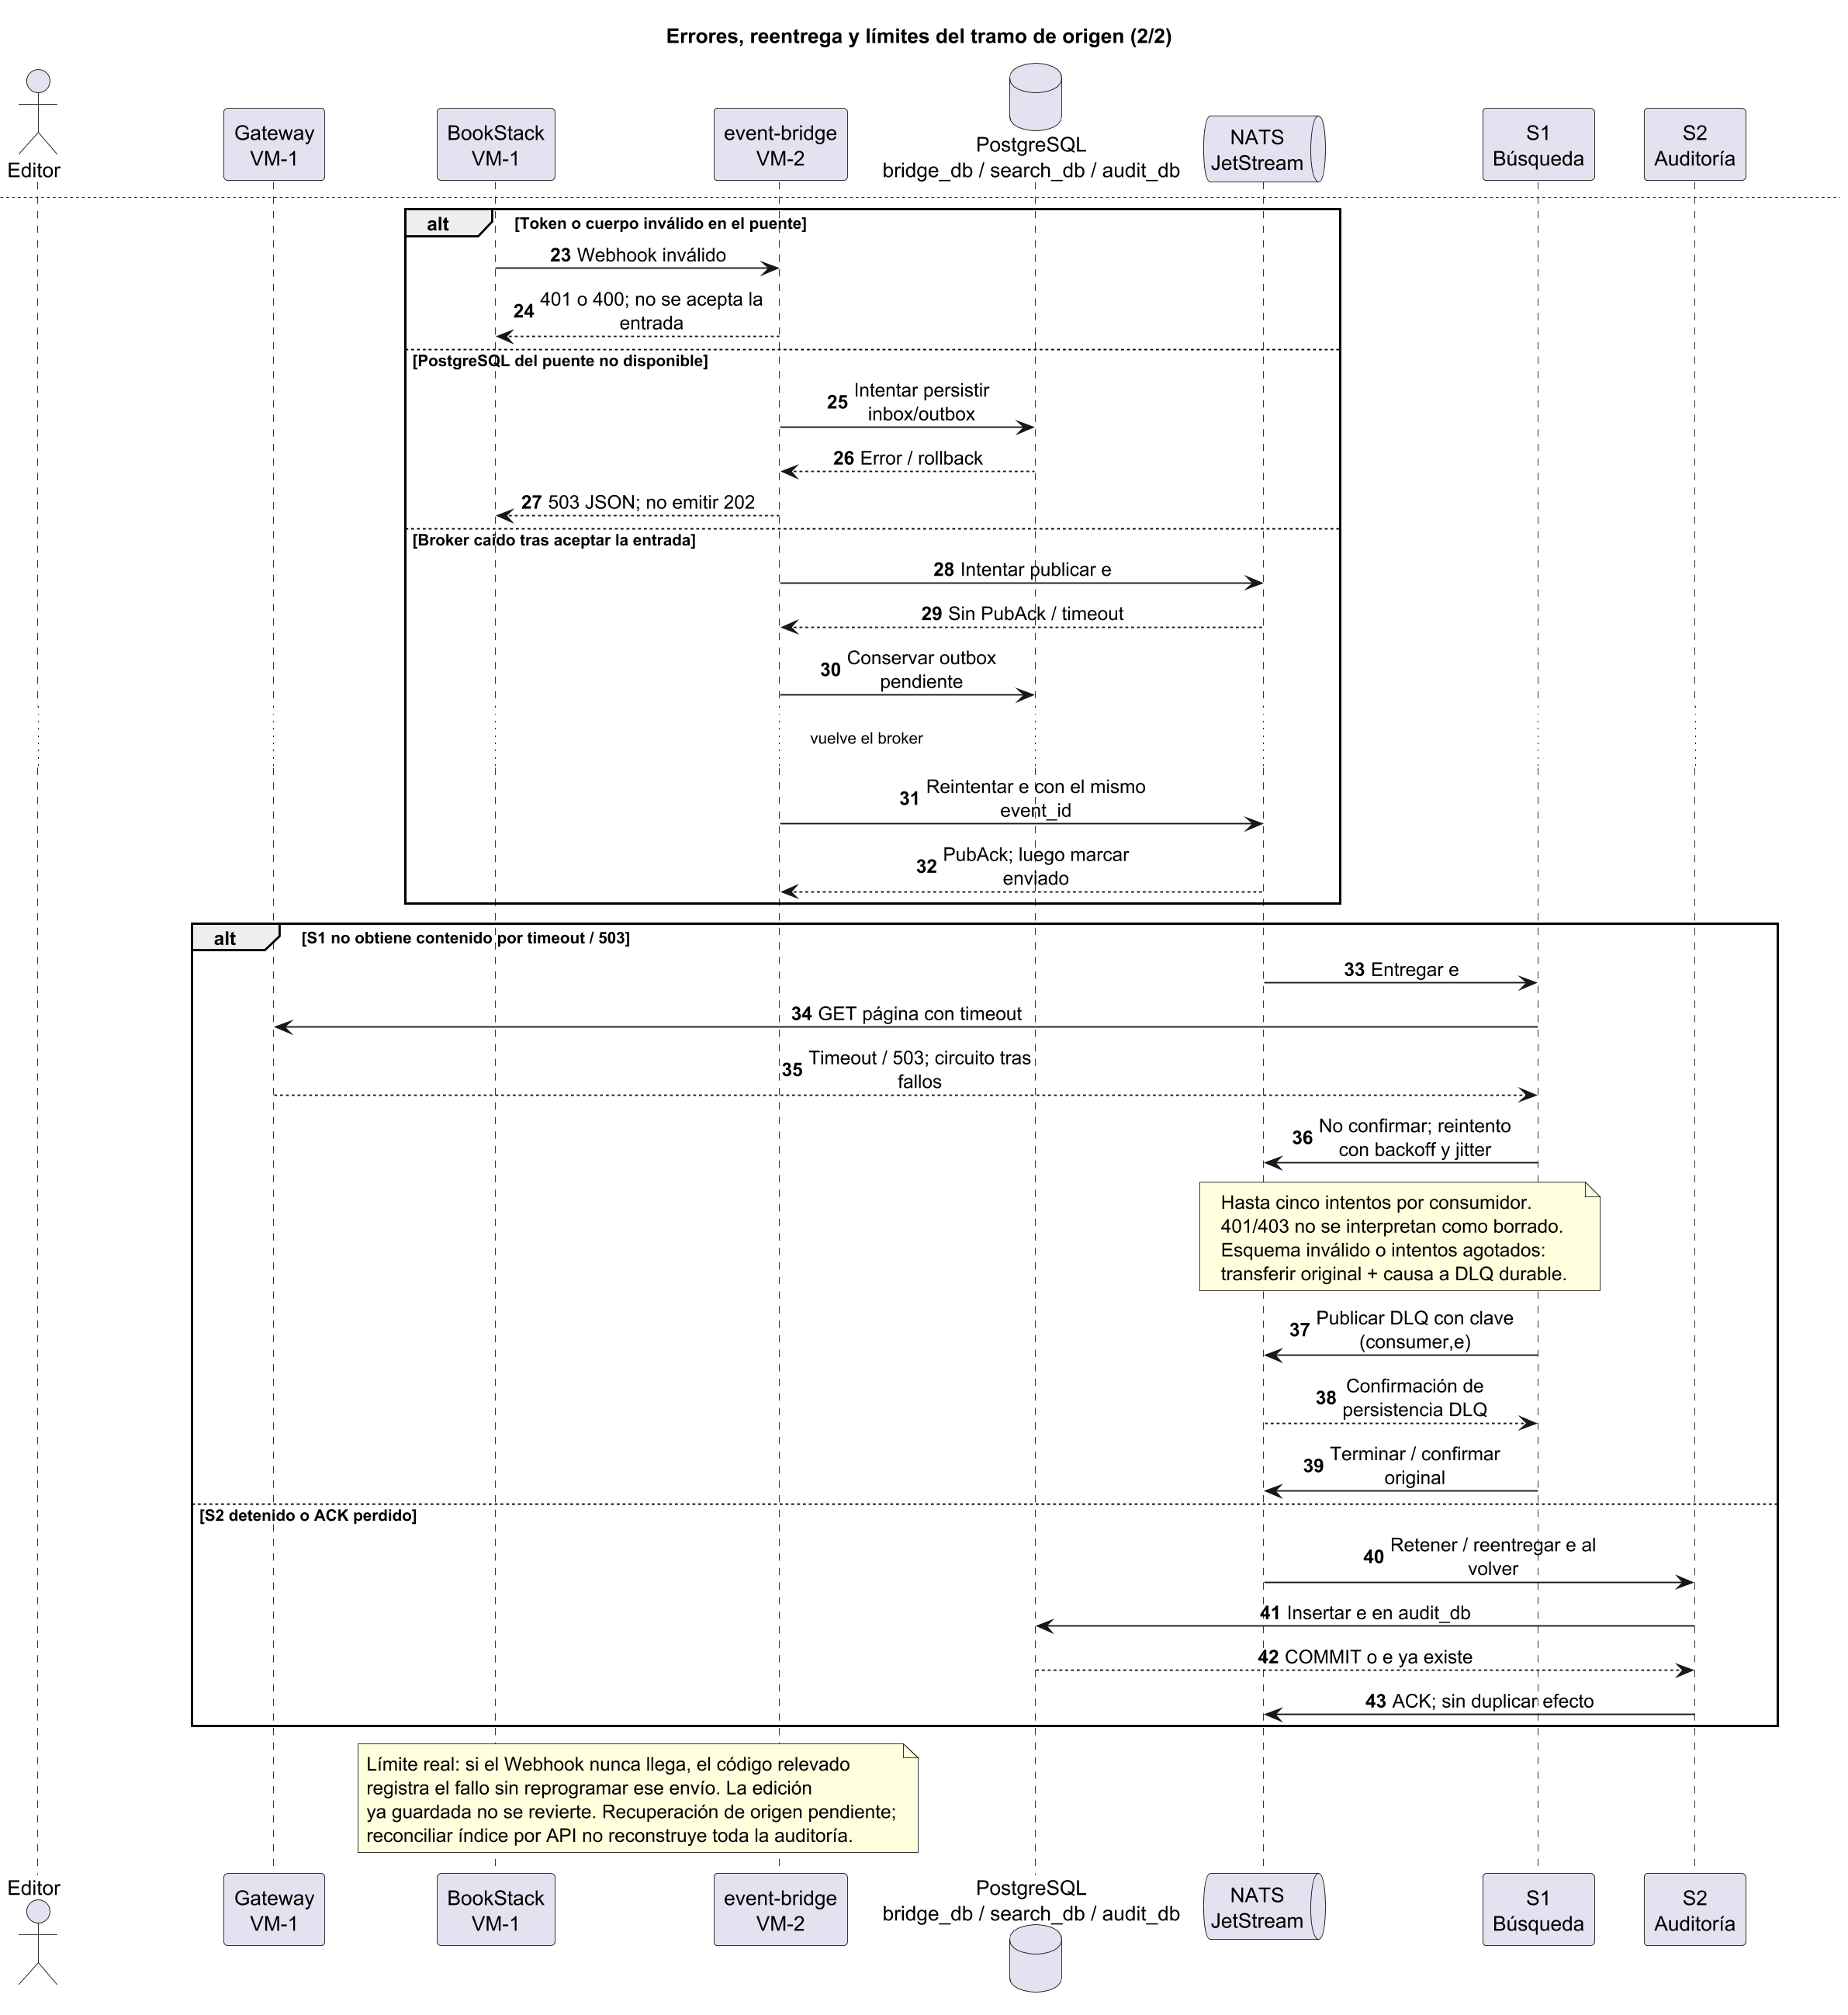
\includegraphics[width=\textwidth,height=0.88\textheight,keepaspectratio]{../../../cna/docs/evidencias/fase5/a4/F5-E7-01-edicion-indexacion_001.png}
\caption{F5-E7 / P32. Secuencia 1, errores y recuperación: outbox, reintentos, DLQ, reentrega y límite de recuperación del Webhook de origen.}
\label{fig:a4-edicion-error}
\end{figure}
\clearpage
\begin{figure}[p]
\centering
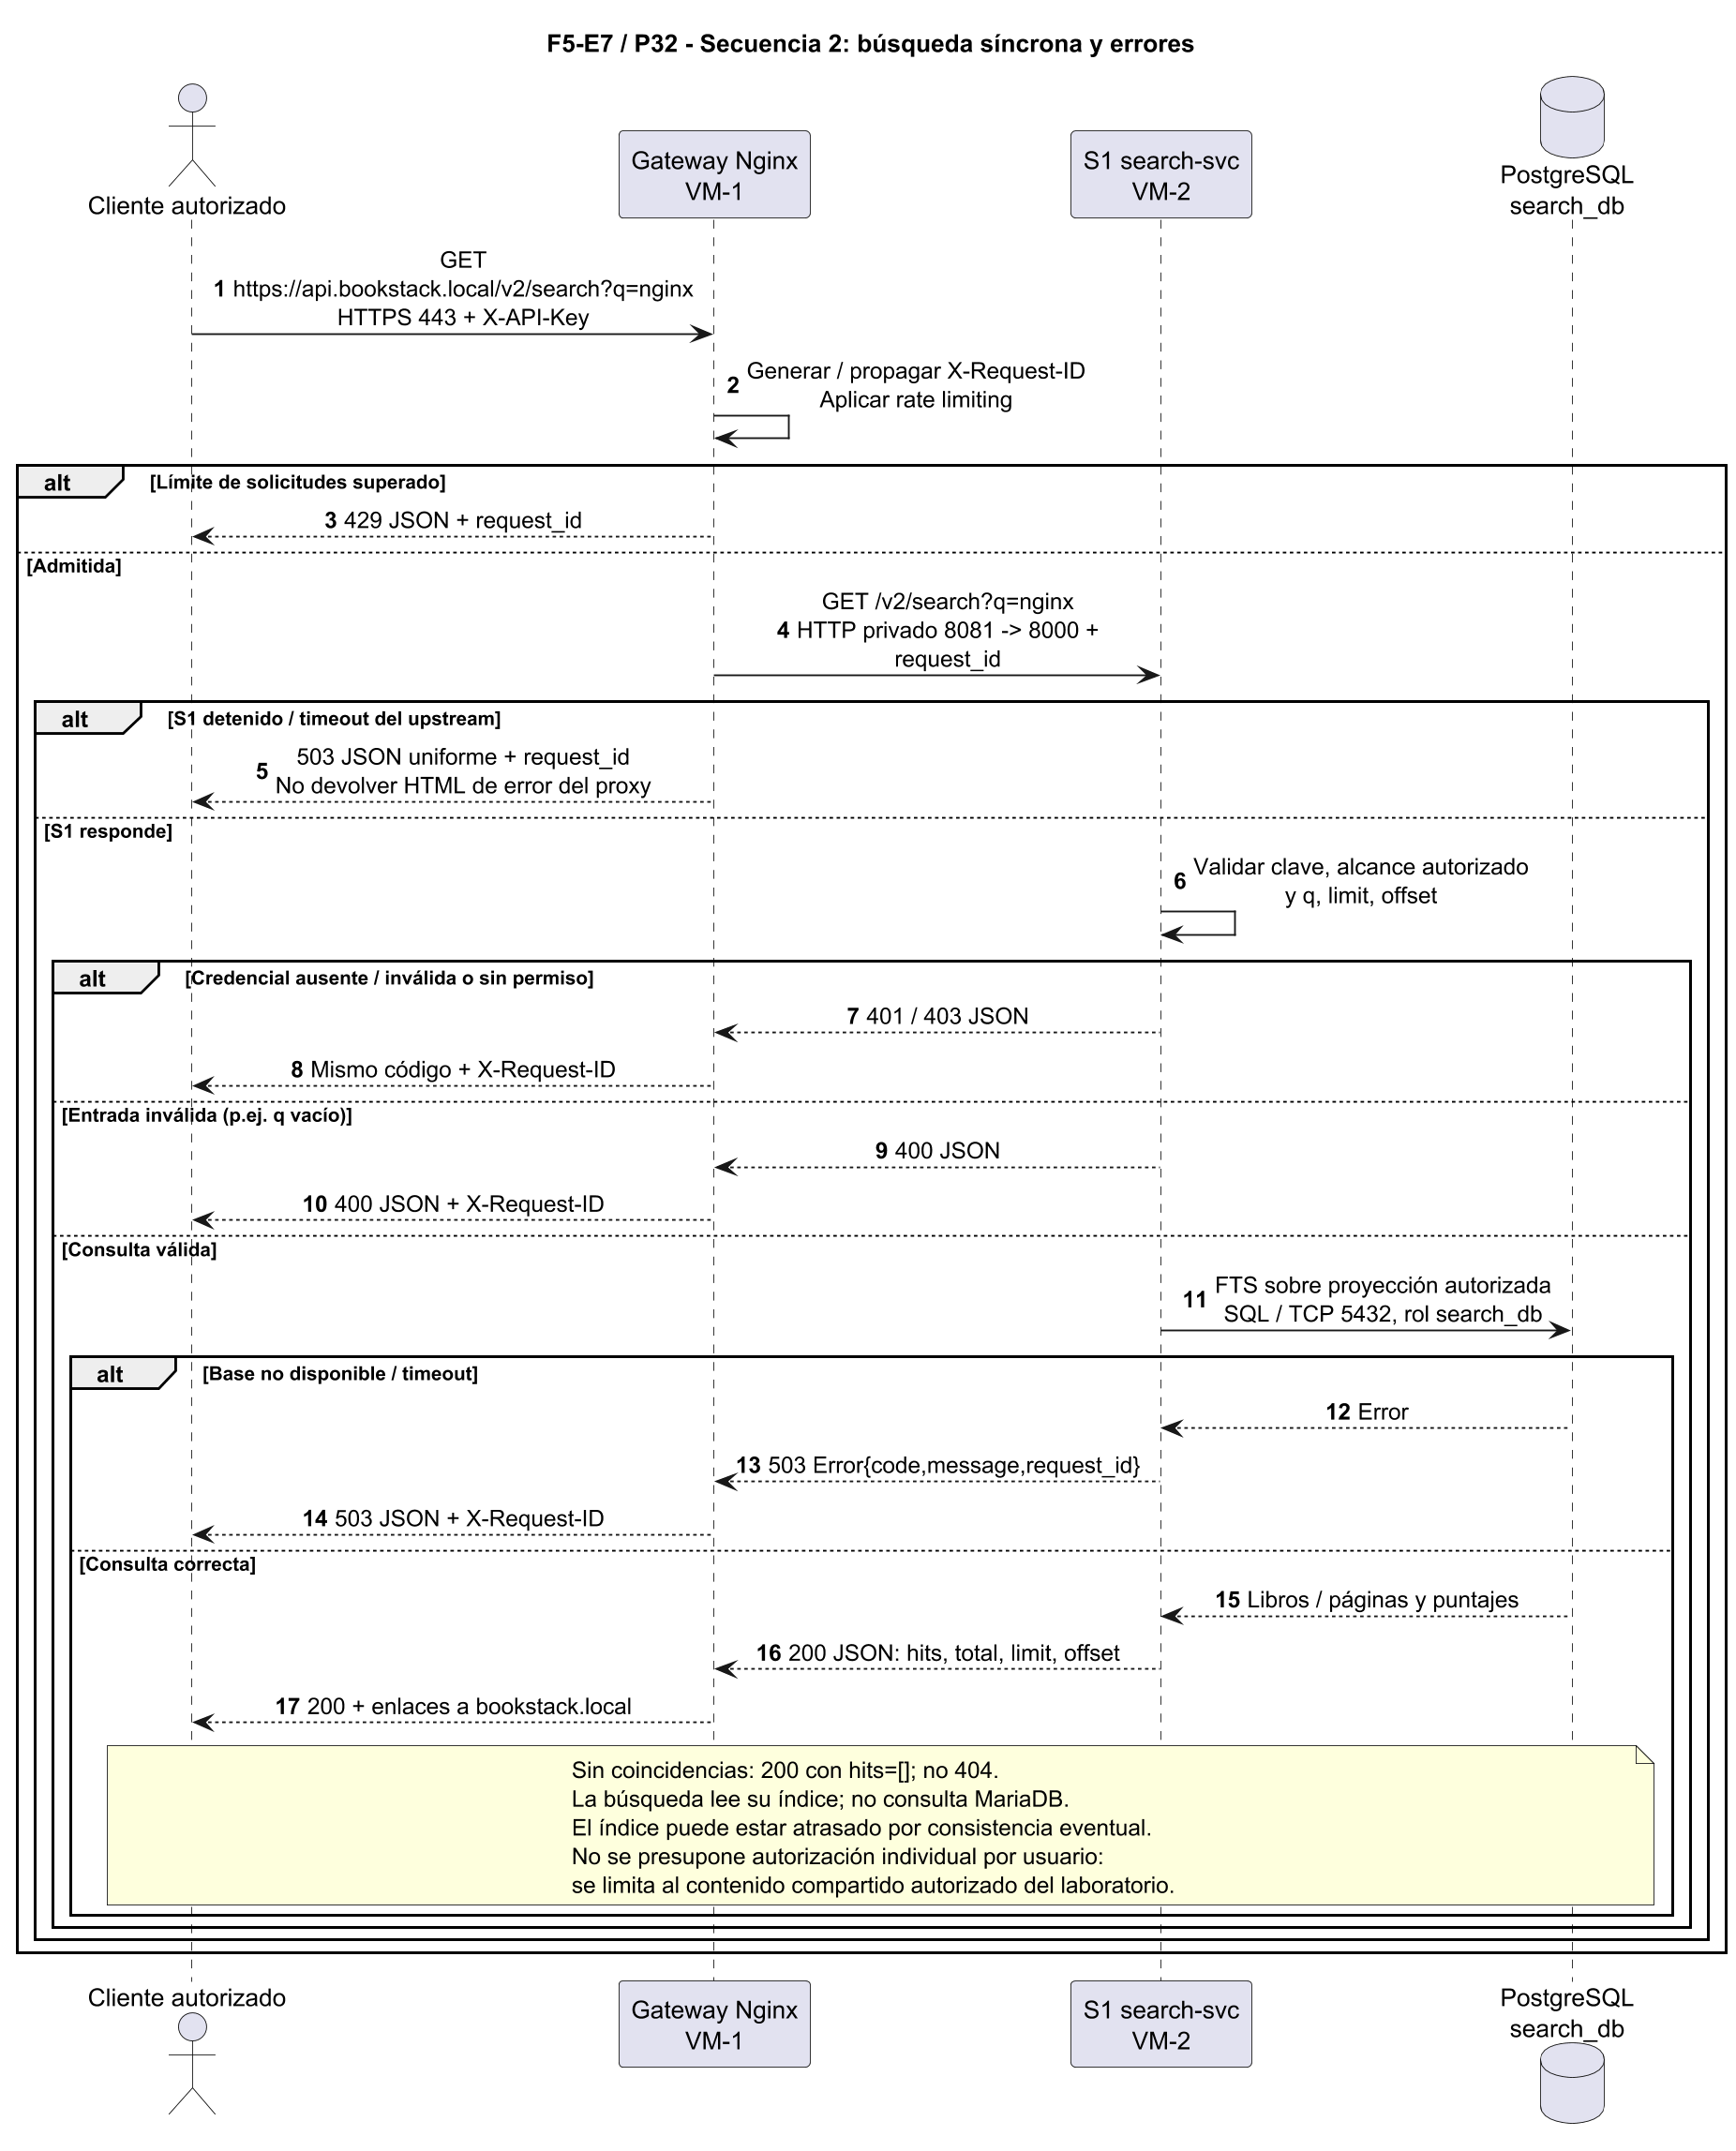
\includegraphics[width=\textwidth,height=0.88\textheight,keepaspectratio]{../../../cna/docs/evidencias/fase5/a4/F5-E7-02-busqueda.png}
\caption{F5-E7 / P32. Secuencia 2: búsqueda síncrona, respuesta normal, validaciones y caminos de error de gateway, servicio e índice.}
\label{fig:a4-busqueda}
\end{figure}
\clearpage
\begin{figure}[p]
\centering
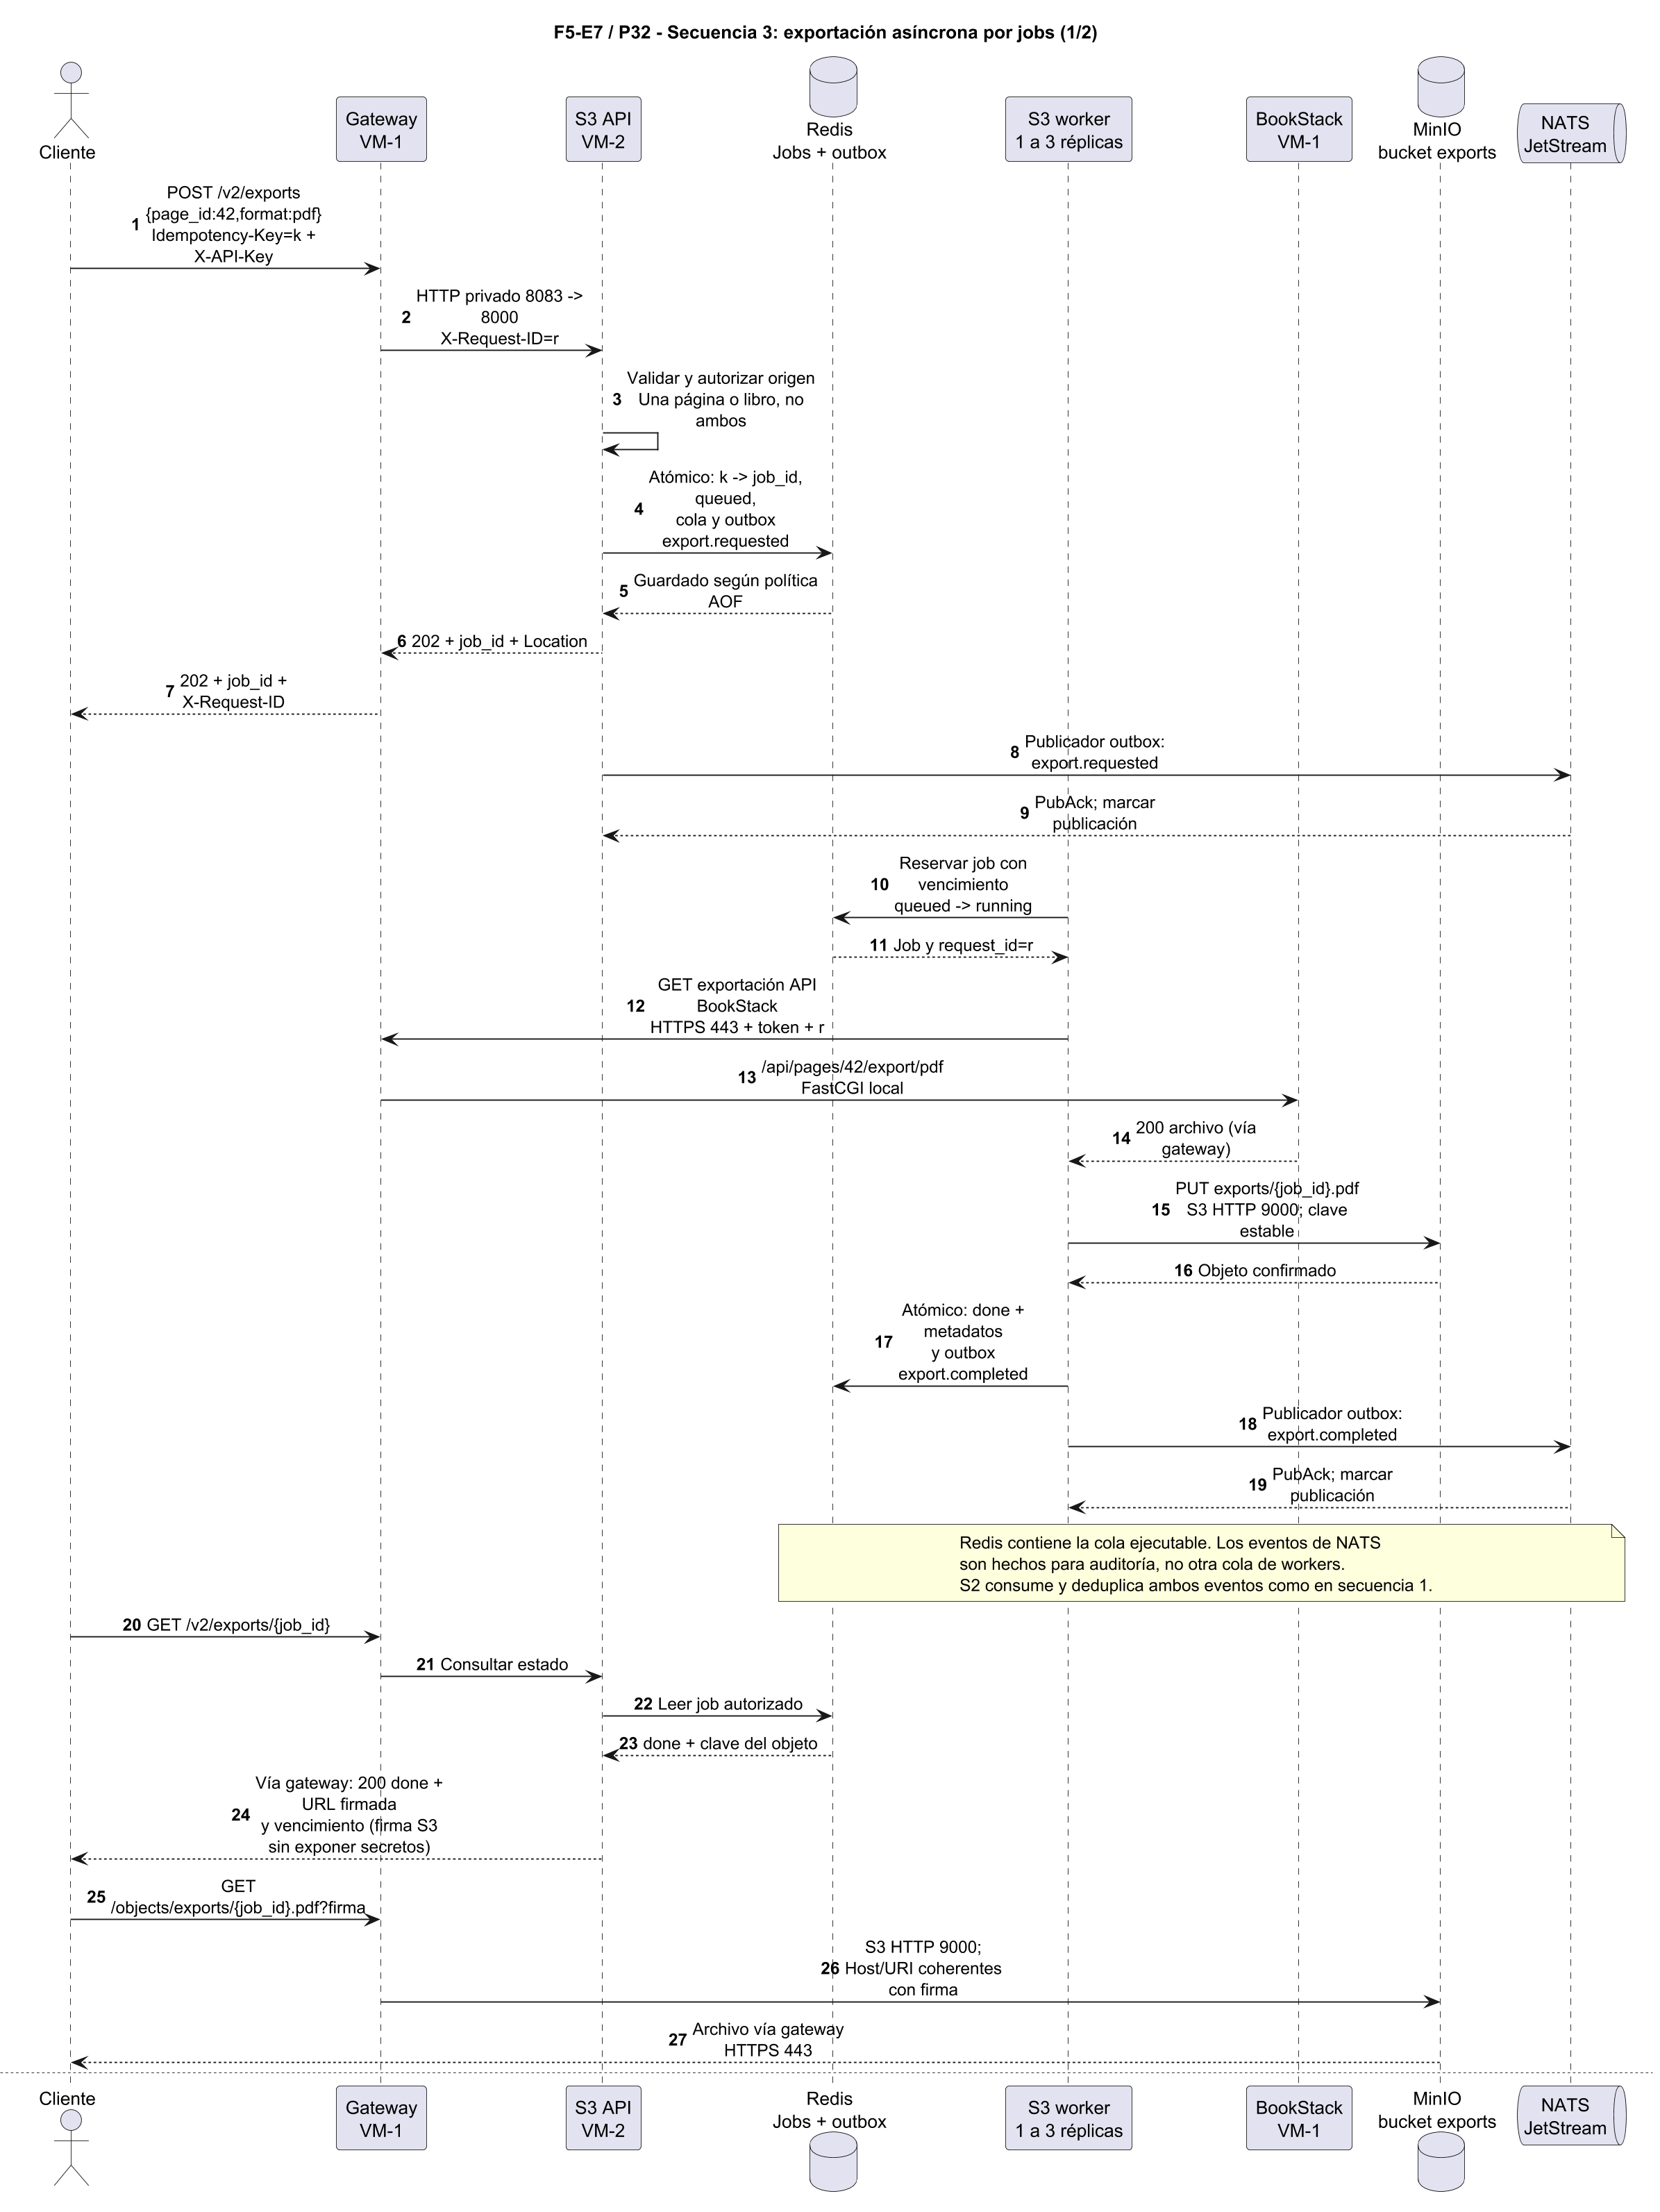
\includegraphics[width=\textwidth,height=0.88\textheight,keepaspectratio]{../../../cna/docs/evidencias/fase5/a4/F5-E7-03-exportacion.png}
\caption{F5-E7 / P32. Secuencia 3, lámina principal: job asíncrono, worker, exportación por API y descarga del objeto mediante URL firmada.}
\label{fig:a4-exportacion}
\end{figure}
\clearpage
\begin{figure}[p]
\centering
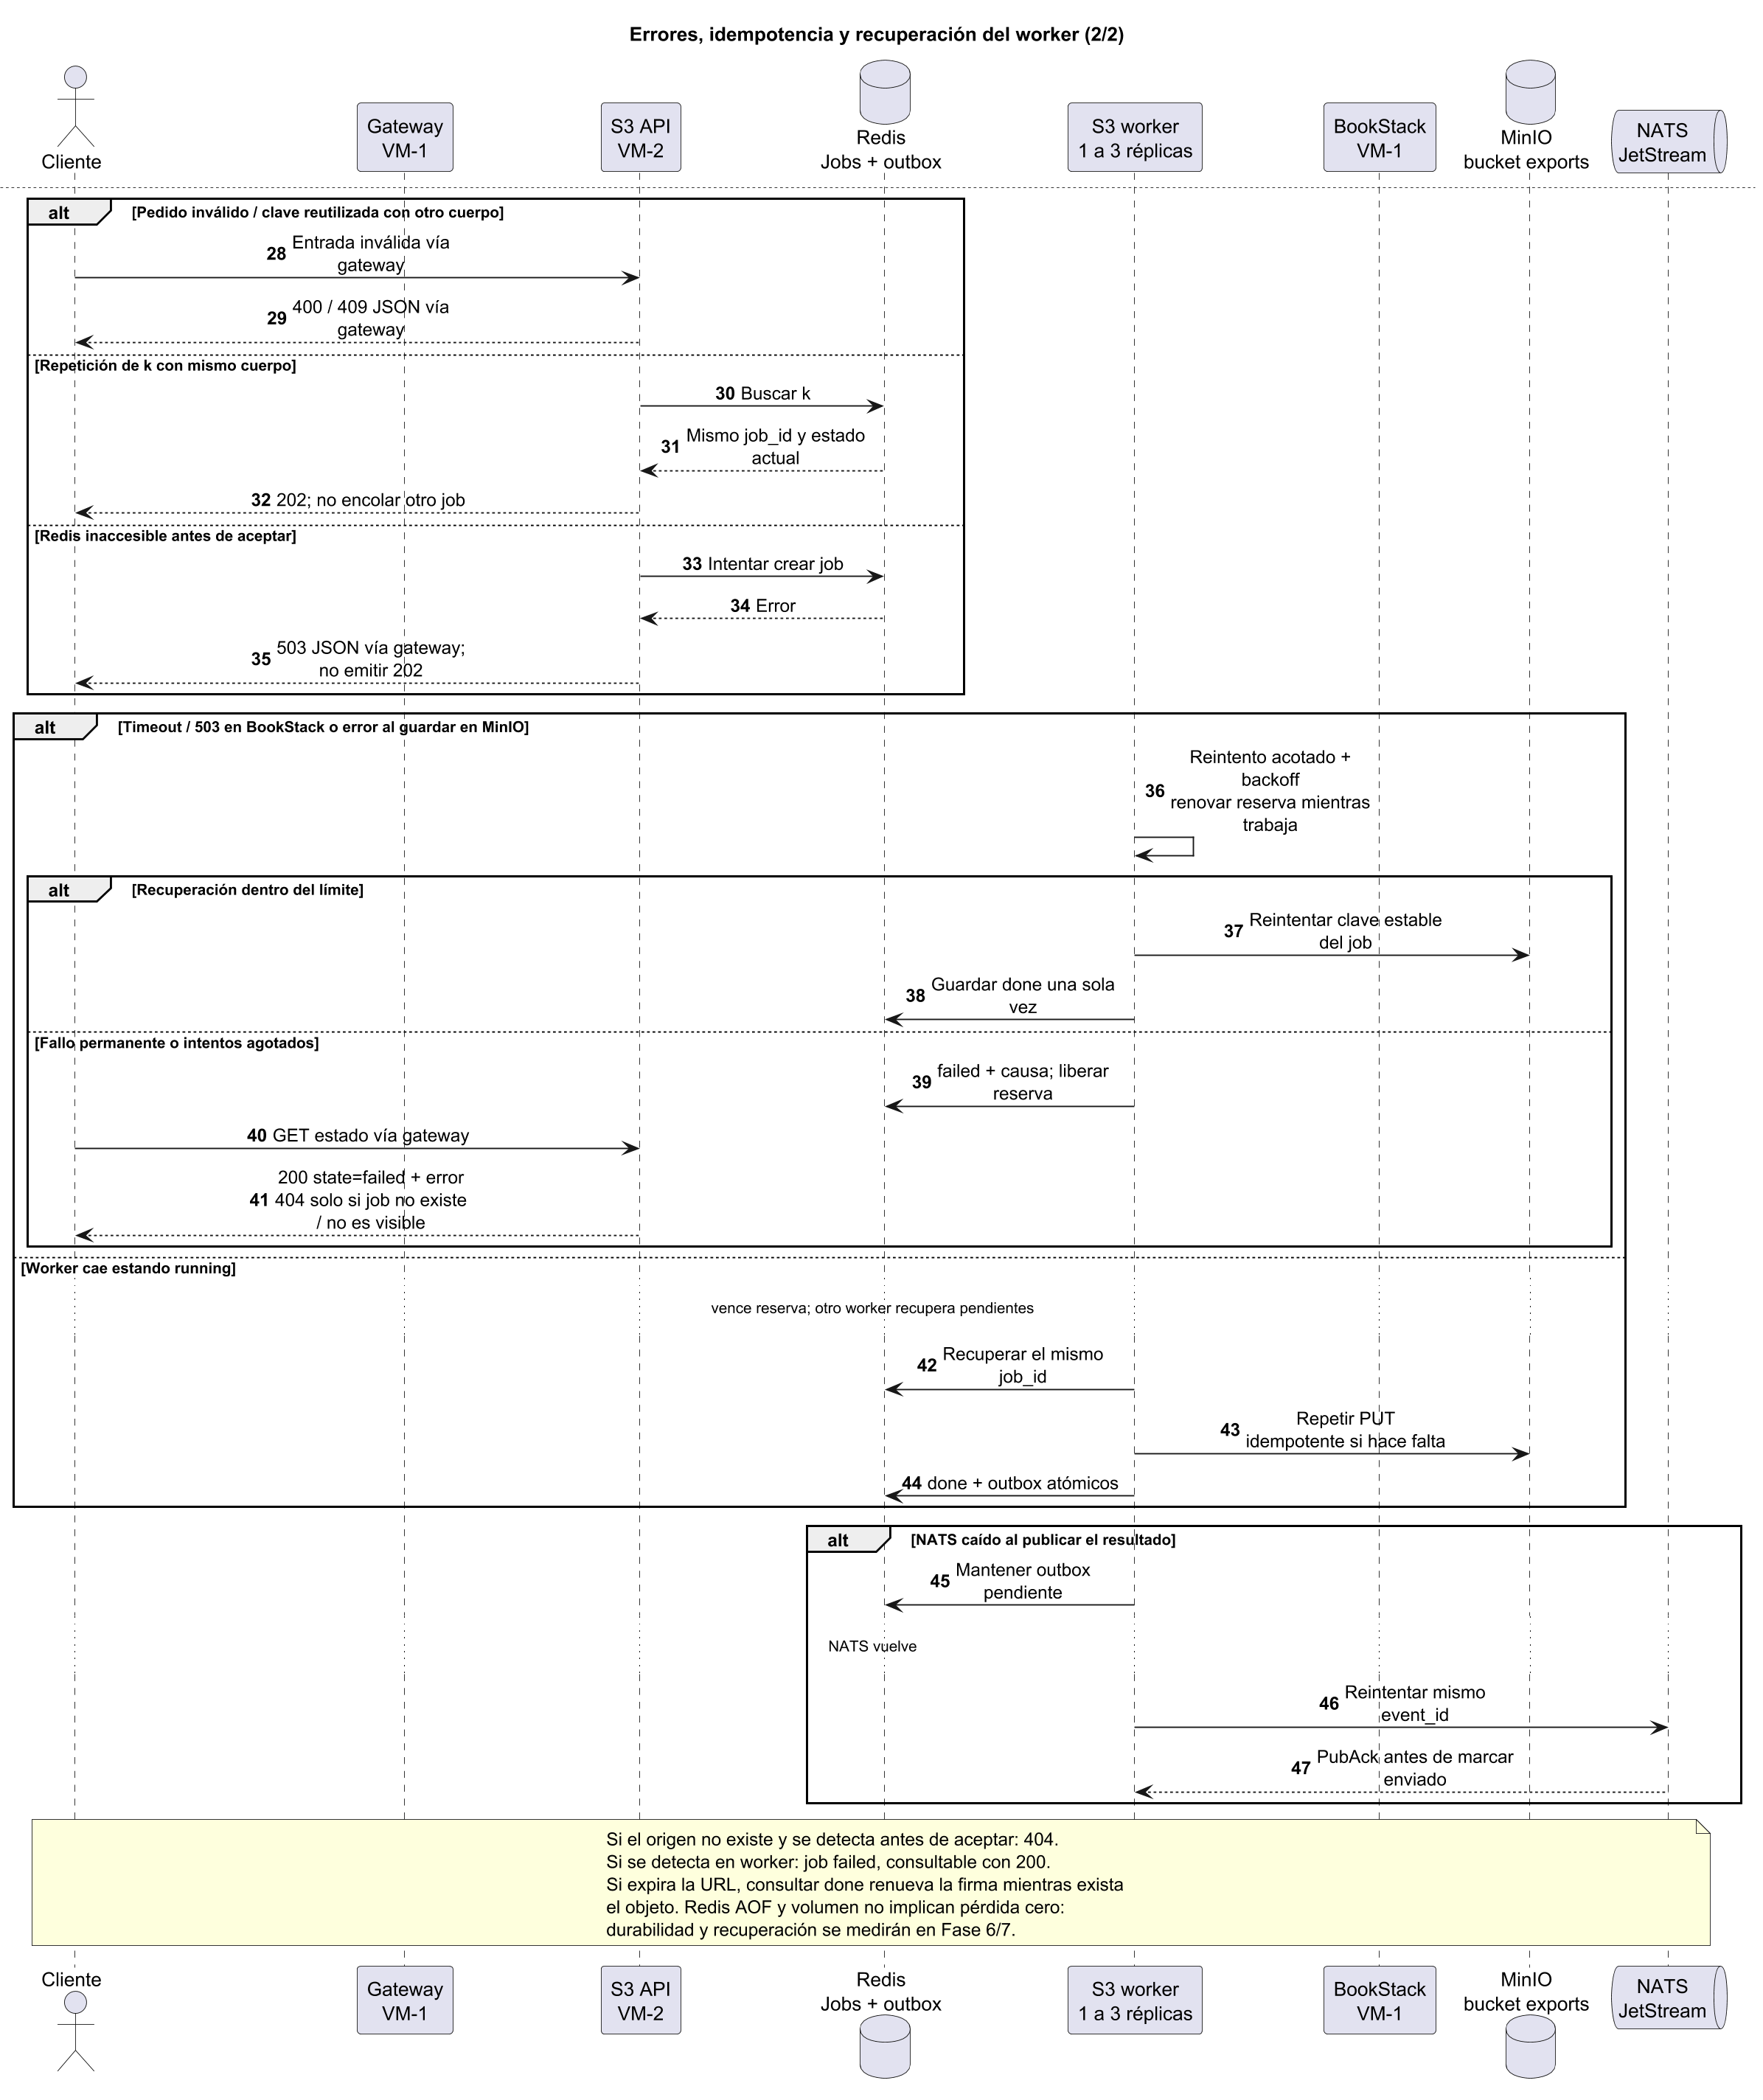
\includegraphics[width=\textwidth,height=0.88\textheight,keepaspectratio]{../../../cna/docs/evidencias/fase5/a4/F5-E7-03-exportacion_001.png}
\caption{F5-E7 / P32. Secuencia 3, errores y recuperación: idempotencia, aceptación condicionada, fallo del worker y publicación recuperable.}
\label{fig:a4-exportacion-error}
\end{figure}
\clearpage

\subsubsection{Fuentes, evidencias y verificación de A4}

Las seis fuentes PlantUML se conservan en
\path{cna/docs/diagramas/a4/}: un contexto, dos vistas del mismo nivel 2 y
tres secuencias. PlantUML 1.2025.10 incluye la biblioteca C4 utilizada;
el script \texttt{renderizar.ps1} comprueba el hash de la herramienta,
la sintaxis y la generación de ocho láminas PNG y ocho SVG. Los SVG conservan
líneas y texto al ampliar y acompañan las imágenes del informe.

Las evidencias y los reportes de compilación se guardan en
\path{cna/docs/evidencias/fase5/a4/}. El JSON registra fecha, nodo, versión
de herramienta y SHA-256 de fuentes y resultados. La revisión visual
comprueba que participantes, alternativas y etiquetas sean legibles y no
estén recortados; la revisión de coherencia contrasta nodos, propiedad de
datos y mensajes con A2 y A3. No constituye una prueba de los servicios.

\begin{table}[H]
\centering\small
\begin{tabularx}{\textwidth}{>{\raggedright\arraybackslash}p{1.3cm} >{\raggedright\arraybackslash}p{1.9cm} X}
\toprule
\textbf{Prueba} & \textbf{Evidencia} & \textbf{Producto de diseño verificado} \\
\midrule
P30 & F5-E5 & C4 nivel 1 con actores, frontera del sistema y accesos. \\
P31 & F5-E6 & Nivel 2 con aplicaciones, almacenes, nodos y puertos/protocolos; vista operativa complementaria. \\
P32 & F5-E7 & Tres interacciones obligatorias, con caminos normales y de error, correlación y recuperación previstas. \\
\bottomrule
\end{tabularx}
\caption{Continuación de la matriz: evidencias de diseño de A4. La comprobación contra el despliegue se realizará en Fase 6.}
\label{tab:a4-evidencias}
\end{table}

La versión de diseño cubre las piezas solicitadas en A4 y conserva las
limitaciones pendientes de implementación. Toda modificación de topología,
puertos o contratos durante la construcción deberá actualizar las fuentes,
regenerar las evidencias y recompilar el informe.
